\documentclass[12pt]{ctexart}
%\usepackage{FRBTemplate}

% ====================基本宏包====================
\usepackage{xeCJK}		% 中文支持
%\usepackage{ctex}
\usepackage{amssymb,amsmath}	% 提供数学符号等支持
\usepackage{color,xcolor}		% 提供颜色支持
\usepackage[bookmarks=true, colorlinks,allcolors=black]{hyperref} % 提供超链接,交叉引用和目录的跳转
% ====================基本宏包====================

% ====================页面格式====================
\usepackage{multicol}	% 分栏
\usepackage{geometry}
\geometry{a4paper}
\geometry{left=3cm,right=2cm,top=2.5cm,bottom=2.5cm}

% 行距
\usepackage{setspace}
\linespread{1.8} 	% 1.8 / 1.2 = 1.5 倍行距(行间距 * 1.2 = 实际行间距)
\setlength{\parskip}{0.5\baselineskip} \newcommand{\setParDis}{\setlength{% 段落间距设置为当前行高的一半
        \parskip}{0pt}} \newcommand{\setParDef}{\setlength{% 使用 \setParDis 将后面段落设为 0 间距
        \parskip}{0.5\baselineskip}}        % 使用 \setParDef 将后面段落设为默认间距

%左右缩进
\usepackage{changepage}

% 页眉页脚
\usepackage{fancyhdr} %页眉页脚
\pagestyle{plain}
\setlength{\headwidth}{\textwidth}	% 页眉长度适应文本
\lhead{}	% 清除左页眉
\rhead{}    % 清除右页眉

% ====================页面格式====================

% ====================字体====================
\usepackage{fontspec}
\setmainfont[													% 西文字体 Times New Roman
    Path				= fonts/,
    BoldFont 			= times-new-roman-bold.ttf,
    ItalicFont 		= times-new-roman-italic.ttf,
    BoldItalicFont 	= times-new-roman-bold-italic.ttf
]{times-new-roman.ttf}
\setmonofont[Path=fonts/]{Courier New.ttf}					% 等宽字体 Courier New
\setCJKfamilyfont{hwzs}[Path=fonts/]{STKzhongsong.ttf}	% 华文中宋
\newcommand{\zhongsong}{\CJKfamily{hwzs}}
\setCJKfamilyfont{hwxw}[Path=fonts/]{STKxinwei.ttf}		% 华文新魏
\newcommand{\xinwei}{\CJKfamily{hwxw}}

% ====================字体====================

% ====================内容强调====================
\usepackage{soul}	% so(字母间隔), caps(全大写), ul(下划线), hl(高亮), st(删除线)
% 可设置 ul,hl,st 颜色:setulcolor{}, sethlcolor{}以及setstcolor{}
% ====================内容强调====================

% ====================代码====================
% 普通代码
\usepackage{listings}

% Python 代码样式
\definecolor{dkgreen}{rgb}{0,0.6,0}	% 需要 xcolor
\definecolor{gray}{rgb}{0.5,0.5,0.5}
\definecolor{mauve}{rgb}{0.58,0,0.82}
\lstset{frame=tb,
    language=Python,
    aboveskip=3mm,
    belowskip=3mm,
    showstringspaces=false,
    columns=flexible,
    basicstyle={\small\ttfamily},
    numbers=left,	%设置行号位置none不显示行号
    %numberstyle=\tiny\courier, 	%设置行号大小
    numberstyle=\tiny\color{gray}, keywordstyle=\color{blue},
    commentstyle=\color{dkgreen}, stringstyle=\color{mauve}, breaklines=true,
    breakatwhitespace=true, escapeinside=``, tabsize=4, extendedchars=false }%逃逸字符显示中文%解决代码跨页时,章节标题,页眉等汉字不显示的问题

%防止伪代码与已有包冲突
\makeatletter
\newif\if@restonecol%
\makeatother
\let\algorithm\relax
\let\endalgorithm\relax
% 伪代码
\usepackage[ruled,linesnumbered]{algorithm2e}
% ruled:标题显示在上面。
% linesnumbered:显示行号。
% boxed:算法放入盒子。
\usepackage{algpseudocode}	%伪代码注释

% 定义 Do-While
\SetKwRepeat{Do}{do}{while}
% 调用方式 \Do{<结束条件>}{<执行命令>}

% 代码块标题
\renewcommand{\lstlistlistingname}{代码汇总}
\renewcommand{\lstlistingname}{代码}
\renewcommand{\algorithmcfname}{算法}

\renewcommand{\algorithmicrequire}{\textbf{Input:}}
\renewcommand{\algorithmicensure}{\textbf{Output:}}
% ====================代码====================

% ====================图表====================
\usepackage{float}		% 浮动体支持
\usepackage{caption}	% 标题
\usepackage{subcaption}	% 子标题
\DeclareCaptionLabelSeparator{mysep}{\space\space}  	%自定义caption格式
\captionsetup[figure]{font={small}, labelfont=bf, labelsep=mysep, textfont={bf}}   	%图片caption格式
\captionsetup[table]{font={small}, labelfont=bf, labelsep=mysep, textfont={bf}}   %表格caption格式

\usepackage{graphicx}		% 插入图片

% 表格
\usepackage{multirow}		% 合并单元格
\usepackage{booktabs}		% 三线表支持

% ====================Tikz====================
\usepackage{tikz,pgfplots}
\pgfplotsset{compat=1.7}
% 不加会出现警告:running in backwards compatibility mode (unsuitable tick labels;
% missing features). Consider writing \pgfplotsset{compat=1.18} into your preamble.
\usetikzlibrary{patterns}
\usetikzlibrary{graphs, positioning, quotes, shapes.geometric,shapes.misc}
% ====================Tikz====================

% ====================目录====================
\setcounter{secnumdepth}{3}		%编号深度
\setcounter{tocdepth}{3}		%目录深度

\renewcommand\listfigurename{插图目录}
\renewcommand\listtablename{表格目录}

% 目录加.....引导符
\usepackage{titletoc} %设置
\titlecontents{section}[1.6em]{\addvspace{2pt}\filright}
{\contentspush{\thecontentslabel\hspace{0.8em}}}
{}{\titlerule*[8pt]{.}\contentspage}

\titlecontents{subsection}[3.2em]{\addvspace{2pt}\filright}
{\contentspush{\thecontentslabel\hspace{0.8em}}}
{}{\titlerule*[8pt]{.}\contentspage}

\titlecontents{subsubsection}[6.4em]{\addvspace{2pt}\filright}
{\contentspush{\thecontentslabel\hspace{0.8em}}}
{}{\titlerule*[8pt]{.}\contentspage}
% ====================目录====================

% ====================其他定义====================
\graphicspath{{image/}}	% 图片路径

\newcommand{\showtitlepage}{
    \thispagestyle{empty}
    \leftline{
\includegraphics{xiaohui.png}}
    \vskip 30pt
        {\centering
            
\includegraphics{xiaoming.png}
            \vskip 12pt
            \zhongsong\zihao{2} 第三十四届“冯如杯”竞赛创意赛道\\
            \vskip 1em
            % 在这写标题,请自行控制标题换行
            一种基于 \LaTeX 的\\
            开源冯如杯论文模板
            \\
            \rightline{\xinwei\zihao{3}{——副标题}}

        }
}

%
\begin{document}

\showtitlepage

%====================摘要====================
\clearpage
\section*{摘要}
\addcontentsline{toc}{section}{摘要}
\begin{spacing}{1.5}
    \setParDis%设置段间距为0
    本项目提出了一种创新的基于三维压电滑台的自制扫描隧道显微镜(STM)设计方案,旨在为科研和教育领域提供一种具有高成本效益、操作简便的纳米级表面分析工具。该设计方案充分考虑了 STM 的核心原理,即量子隧道效应,以及实现原子级别分辨率成像所需的关键组件,包括探针、样品台、压电陶瓷扫描器、反馈控制系统和真空系统。我们详细讨论了在设计和构建过程中遇到的技术难点,例如如何制备具有纳米级锐度的探针、如何精确控制极小隧穿电流以及如何实现探针的纳米级精确移动。

    为了解决这些挑战,我们采用了先进的电子电路设计,包括高精度的前置放大器和数字模拟转换器,以及基于 STM32F103C8T6 微控制器的固件程序。控制软件采用Python语言开发,提供友好的用户界面和强大的数据处理功能,能够将隧穿电流信号转换为样品表面的二维与三维图像。

    此外,我们还探讨了自制STM在纳米科学、新材料开发、表面科学研究以及教育领域的广泛应用前景。在市场需求与商业化方面,我们分析了自制 STM 相对于市场上现有产品的竞争优势,并讨论了如何通过与工业界的合作,将这一技术转化为具有商业价值的产品。

    最后,我们对自制 STM 的优劣进行了分析,并提出了未来优化的方向,包括提高系统的稳定性和可靠性,以及开发更加直观易用的用户界面。通过开源与社区合作,我们相信自制 STM 项目能够激发更广泛的科学兴趣,促进科学知识的传播和技术的创新。

\end{spacing}

\textbf{关键词:}扫描隧道显微镜(STM),三维压电滑台,低成本,科研工具,教育应用,开源硬件
%====================摘要====================

%====================目录====================
\clearpage
% 普通目录
\tableofcontents
\addcontentsline{toc}{section}{目录}    %添加目录到目录
% 插图目录
{
    \let\oldnumberline\numberline%
    \renewcommand{\numberline}{\figurename~\oldnumberline}%
    \listoffigures
    \addcontentsline{toc}{section}{插图目录}
}
% 表格目录
{
    \let\oldnumberline\numberline%
    \renewcommand{\numberline}{\tablename~\oldnumberline}%
    \listoftables
    \addcontentsline{toc}{section}{表格目录}
}
%====================目录====================

%====================正文====================
\section{引言}

\section{图表示例}

\begin{figure}[htbp]
    \begin{subfigure}{0.31\textwidth}
        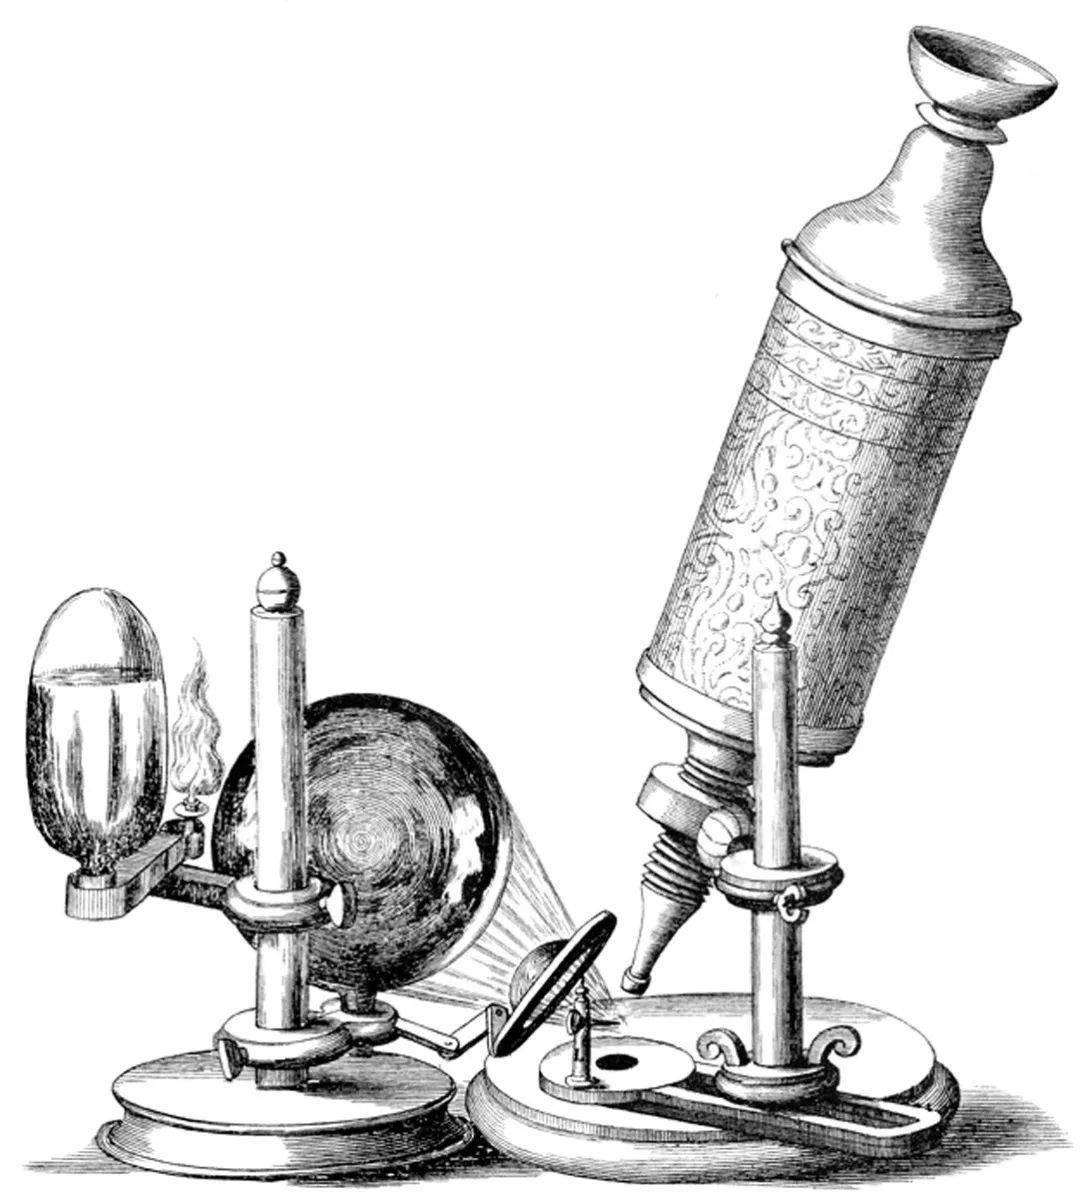
\includegraphics[width=\linewidth]{fig1.jpeg}
        \caption{Robert Hooke 制作的复合显微镜}
    \end{subfigure}%
    \hfill
    \begin{subfigure}{0.31\textwidth}
        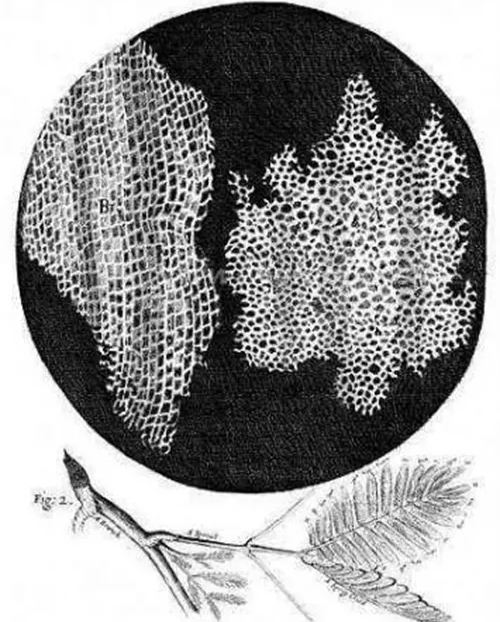
\includegraphics[width=\linewidth]{fig2.png}
        \caption{Robert Hooke 观察栎树皮薄片}
    \end{subfigure}
    \hfill
    \begin{subfigure}{0.31\textwidth}
        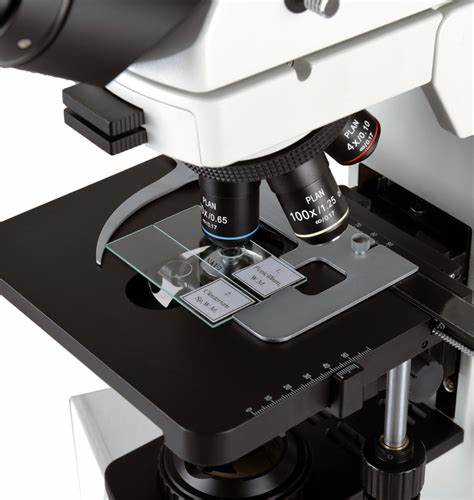
\includegraphics[width=\linewidth]{fig3.png}
        \caption{现代光学显微镜}
    \end{subfigure}
    \caption{显微镜的发展历史:光学显微镜}
\end{figure}
\vskip 1em

\begin{table}[!h]
    \small
    \caption{DIY-STM 接线表}
    \centering
    \begin{tabular}{ccccc}
        \toprule[1.5pt]
        \textbf{\quad 源 PCB\quad}        & \textbf{\quad 目标 PCB\quad}      & \textbf{\quad 源接口\quad} & \textbf{\; 目标接口\;} & \textbf{\quad 类型\quad}   \\
        \midrule[0.8pt]
        Power\_Board                     & Motor\_Board                    & 3V3\_1                  & 3V3                & MMCX-MMCX                \\
        Power\_Board                     & Motor\_Board                    & +12                     & +12V               & MMCX-MMCX                \\
        Power\_Board                     & Motor\_Board                    & -12                     & -12V               & MMCX-MMCX                \\
        Power\_Board                     & Motor\_Board                    & +15\_1                  & +15V               & MMCX-MMCX                \\
        Power\_Board                     & Motor\_Board                    & -15\_1                  & -15V               & MMCX-MMCX                \\
        \midrule[0.1pt]
        Power\_Board                     & Controller\_Board               & 3V3\_2                  & 3V3                & MMCX-MMCX                \\
        Power\_Board                     & Controller\_Board               & +15\_2                  & +15V               & MMCX-MMCX                \\
        Power\_Board                     & Controller\_Board               & -15\_2                  & -15V               & MMCX-MMCX                \\
        Power\_Board                     & Controller\_Board               & +15\_3                  & +15V               & MMCX-MMCX                \\
        Power\_Board                     & Controller\_Board               & -15\_3                  & -15V               & MMCX-MMCX                \\
        \midrule[0.1pt]
        Power\_Board                     & ADC\_And\_MCU\_Board            & 3V3\_3                  & 3V3                & MMCX-MMCX                \\
        Power\_Board                     & ADC\_And\_MCU\_Board            & 5V                      & 5V                 & MMCX-MMCX                \\
        \midrule[0.1pt]
        Motor\_Board                     & ADC\_And\_MCU\_Board            & SPI2                    & SPI2               & IDC-IDC$^\text{1}$       \\
        Controller\_Board                & ADC\_And\_MCU\_Board            & SPI1                    & SPI1               & IDC-IDC                  \\
        \midrule[0.1pt]
        Power\_Board                     & Connector\_Board                & +15\_4                  & +15V               & MMCX-MMCX                \\
        Power\_Board                     & Connector\_Board                & -15\_4                  & -15V               & MMCX-MMCX                \\
        Power\_Board                     & Connector\_Board                & GND                     & GND                & MMCX-MMCX                \\
        \midrule[0.1pt]
        Motor\_Board                     & PZT\_Slide\_Table               & X / Y / Z               & X / Y / Z          & MMCX-MMCX                \\
        \multirow{2}*{Controller\_Board} & \multirow{2}*{Connector\_Board} & Z+X / Z-X               & Z+X / Z-X          & \multirow{2}*{MMCX-MMCX} \\
        ~                                &                                 & Z+Y / Z-Y               & Z+Y / Z-Y          &                          \\
        \midrule[0.1pt]
        Connector\_Board                 & ADC\_And\_MCU\_Board            & ADC                     & ADC\_IN            & MMCX-MMCX                \\
        \bottomrule[1.5pt]
    \end{tabular}
    \\\vskip 1mm
    \begin{minipage}{0.95\linewidth}
        附注 1:IDC 插头型号为:2.54-2$\times$5P。
    \end{minipage}
    \label{tab2}
\end{table}
\vskip 1em

\section{用法参考}
\subsection{伪代码}
使用 Algorithm2e 宏包实现。

\begin{algorithm}[!h]
    \KwData{this text}
    \KwResult{how to write algorithm with \LaTeX2e }
    initialization\;
    \While{not at end of this document}{
        read current\;
        \Repeat{this end condition}{
            do these things\;
        }
        \eIf{understand}{
            go to next section\;
            current section becomes this one\;
        }{
            go back to the beginning of current section\;
        }
        \Do{this end condition}{
            do these things\;
        }
    }
    \caption{How to write algorithms}
\end{algorithm}

\end{document}
